\def\filepath{/home/stephenmalina/dev/templates}

%http://web.mit.edu/rsi/www/pdfs/beamer-tutorial.pdf
\documentclass[pdf]{beamer} %
\mode<presentation>{\usetheme{Boadilla}}
\bibliographystyle{acm}

\input{\filepath/packages_beamer.tex}
\input{\filepath/macros.tex}


\setbeamertemplate{itemize items}[default]
\setbeamertemplate{enumerate items}[default]
\setbeamertemplate{section in toc}{%
  {\inserttocsectionnumber.}~\inserttocsection}
\setbeamertemplate{subsection in toc}{%
  \hspace{1.2em}{\rule[0.3ex]{3pt}{3pt}}~\inserttocsubsection\par}
\setbeamertemplate{subsubsection in toc}{%
  \hspace{2.4em}{\rule[0.3ex]{3pt}{3pt}}~\inserttocsubsubsection\par}


\AtBeginSection[]{
  \begin{frame}
  \vfill
  \centering
  \begin{beamercolorbox}[sep=8pt,center,shadow=true,rounded=true]{title}
    \usebeamerfont{title}\insertsectionhead\par%
  \end{beamercolorbox}
  \vfill
  \end{frame}
}
\title{Deep MR\footnote{Title is a WIP.}}
\subtitle{Interrogating Deep Learning Models with Mendelian Randomization}
\author{Stephen Malina in collaboration with David Knowles and Daniel Cizin}

\begin{document}
\begin{frame}
\titlepage
\end{frame}
%% normal frame
\begin{frame}{Outline}
    \begin{block}{Disclaimer}
        I made this presentation more provocative than usual. I apologize in advance...
    \end{block}
    \tableofcontents
\end{frame}

\section{Motivation}
\subsection{Machine Learning Perspective}
 
\begin{frame}[t]{ML perspective: Do deep learning models learn causal relationships?}
    
    \begin{columns}
        \column{.5\textwidth}
        If I train my deep learning model to jointly predict two processes one of which causes the other, will it learn the causal relationship between the two?
        \column{.5\textwidth}
    \begin{figure}[htpb]
        \centering
        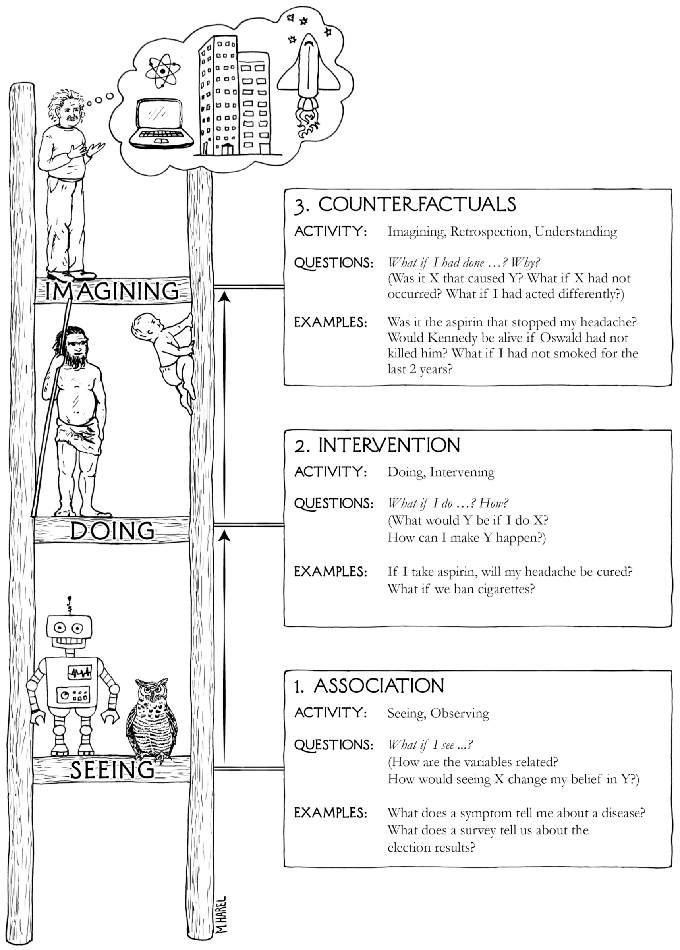
\includegraphics[width=0.7\linewidth]{figures/ladder_of_causation}
        \label{fig:ladder_of_causation}
    \end{figure}
    \end{columns}

\end{frame}

\subsection{Biology Perspective}
\begin{frame}[t]{Biology Perspective: Microscope Models\footnote{Stolen from Chris Olah}}
   \begin{block}{Pretend you're a biologist...}
      If you're a biologist, pretend you're a `pretend biologist'. 
   \end{block} 

   Imagine a model of a complex process like splicing plus RBP binding that you can use to:
   \begin{enumerate}
       \item Ask questions about / verify underlying mechanisms
       \item Generate hypotheses for mysterious things to look into
   \end{enumerate}
   \textit{Without our help!}

   \begin{block}{Claim} We are far from this... Why? Lots of reasons! \end{block}
\end{frame}

\begin{frame}[t]{Slicing off a piece of the problem}
%     \begin{block}{Promise of black box (e.g.\ deep learning) models}
%         If `representation learning' works, then our models can become like microscopes (stolen from Chris Olah) which we can use to understand mechanism
%     \end{block}
    One way to try and better understand what our models have learned: look at whether they model the `correct' relationships between different processes.
\end{frame}

% \begin{frame}[t]{Increasing Confidence in our\footnote{ML folks'} Models}
%     \begin{itemize}
%         \item Increasing amount of work~\cite{zhou2015predicting, Shrikumar2017-uj} trying to understand what models learn at the individual input level and output level
%         \begin{itemize}
%             \item Use `in-silico' mutagenesis to test whether mutations have the expected effect
%         \end{itemize}
%         \item Also some~\cite{zhou2015predicting, Koo2018-cb} trying to analyze what models learn at a higher level
%         \item But these works:
%         \begin{itemize}
%             \item Lack a principled framework for determining whether effects are meaningful
%             \item Don't look at relationships between processes
%         \end{itemize}
%     \end{itemize}
% \end{frame}
% 
% \begin{frame}[t]{From Hypothesis Verification to Generation}
%     Existing methods~\cite{zhou2015predicting, Koo2018-cb, Shrikumar2017-uj} limit themselves to: 
%     \begin{enumerate}
%         \item Answering human-defined queries about individual processes
%             \begin{itemize}
%                 \item Does mutating this nucleotide increase the probability of binding?
%                 \item Does binding probability for this sequence respond to changes in any nucleotide within it?
%             \end{itemize}
%         \item Verifying the effect of mutations on sequences where we know they have an effect
%     \end{enumerate}
% \end{frame}

\begin{frame}[t]{Recap}
    \begin{block}{Clarification} All the work I've mentioned so far is great! Haven't talked about generative models, but they try to solve some of these problems. \end{block}
    \begin{block}{Summary}
    \begin{itemize}
        \item Complex models that work are great
        \item Maximizing the value we get from complex models requires better techniques for understanding what they've learned
    \end{itemize}
    \end{block}
    \begin{block}{Looking ahead}
        Leveraging tools from causal inference to better understand what our models have learned.
    \end{block}
\end{frame}

\section{Background}
\subsection{Causal Inference \& Mendelian Randomization}
\begin{frame}{Causal Inference \& Mendelian Randomization}
    To the whiteboard!
\end{frame}

\subsection{Deep learning for functional 'omics prediction}
\begin{frame}[t]{Deep learning for DNA/RNA sequence-specific prediction}
    \begin{itemize}
        \item Tons of work using CNNs/RNNs/etc.\ to predict biological processes from sequence
        \item Examples include:
        \begin{itemize}
            \item Transcription factor (TF) binding~\cite{alipanahi2015predicting, zhou2015predicting}
            \item Chromatin accessibility (CA)~\cite{zhou2015predicting, kelley2016basset}
            \item RNA binding protein (RBP) binding~\cite{zheng2018deep, Koo2018-cb}
        \end{itemize}
        \item We'll focus on first two but method in principle applies any time we have two causally related processes we're jointly modeling
    \end{itemize}
\end{frame}

\begin{frame}[t]{Interpretability, briefly}
    Two high-level approaches to understanding what sequence predictor networks have learned:
    \begin{enumerate}
        \item In-silico mutagenesis (see~\cite{zhou2015predicting, kelley2016basset})
            \begin{itemize}
                \item Take a sequence from your test set
                \item Mutate it
                \item See how the predictions change
            \end{itemize}
        \item Gradient-based approaches (see~\cite{Shrikumar2017-uj, Simonyan2013-xy})
            \begin{itemize}
                \item Make a prediction for a sequence
                \item Look at gradient of the loss w.r.t.\ (some function of) input
            \end{itemize}
    \end{enumerate}
\end{frame}

\subsection{Biology}
\begin{frame}[t]{Transcription factors regulate accessibility \& protein production}
    \begin{figure}[htpb]
        \centering
        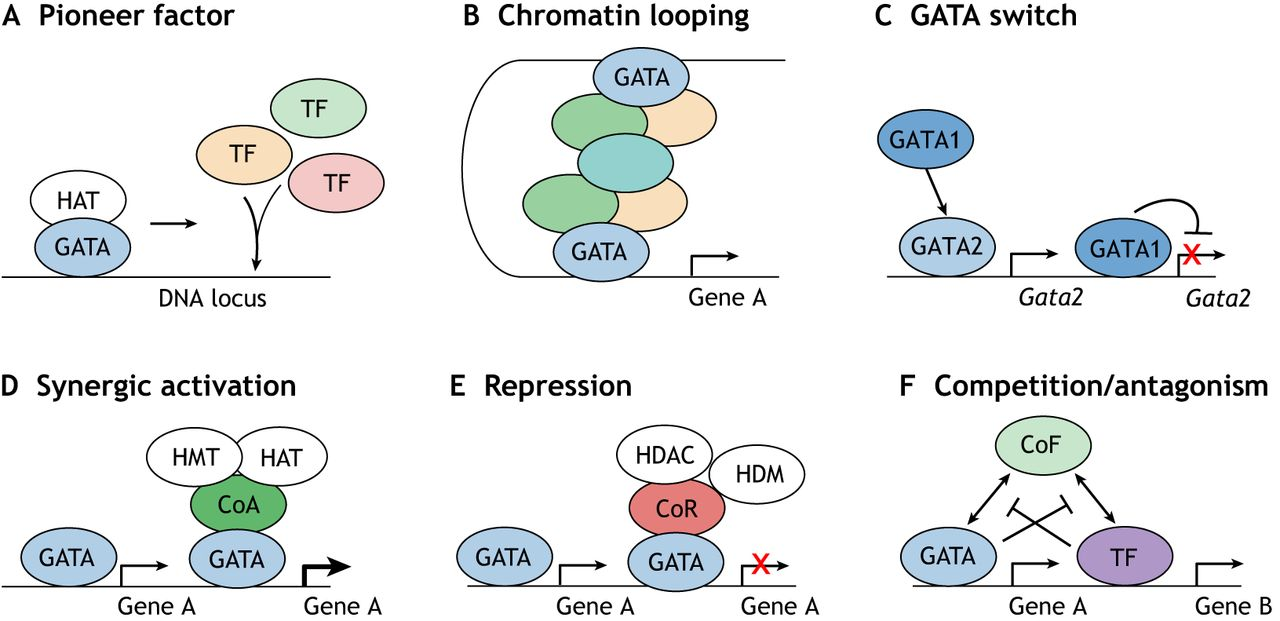
\includegraphics[width=0.8\linewidth]{figures/tf_explanation}
        \caption{Six mechanisms through which transcription factor binding can regulate transcription\cite{Tremblay2018-ds}.}
        \label{fig:tf_explanation}
    \end{figure} 
\end{frame}

\begin{frame}[t]{Measuring transcription factor binding with ChIP-seq}
    \begin{figure}[htpb]
        \centering
        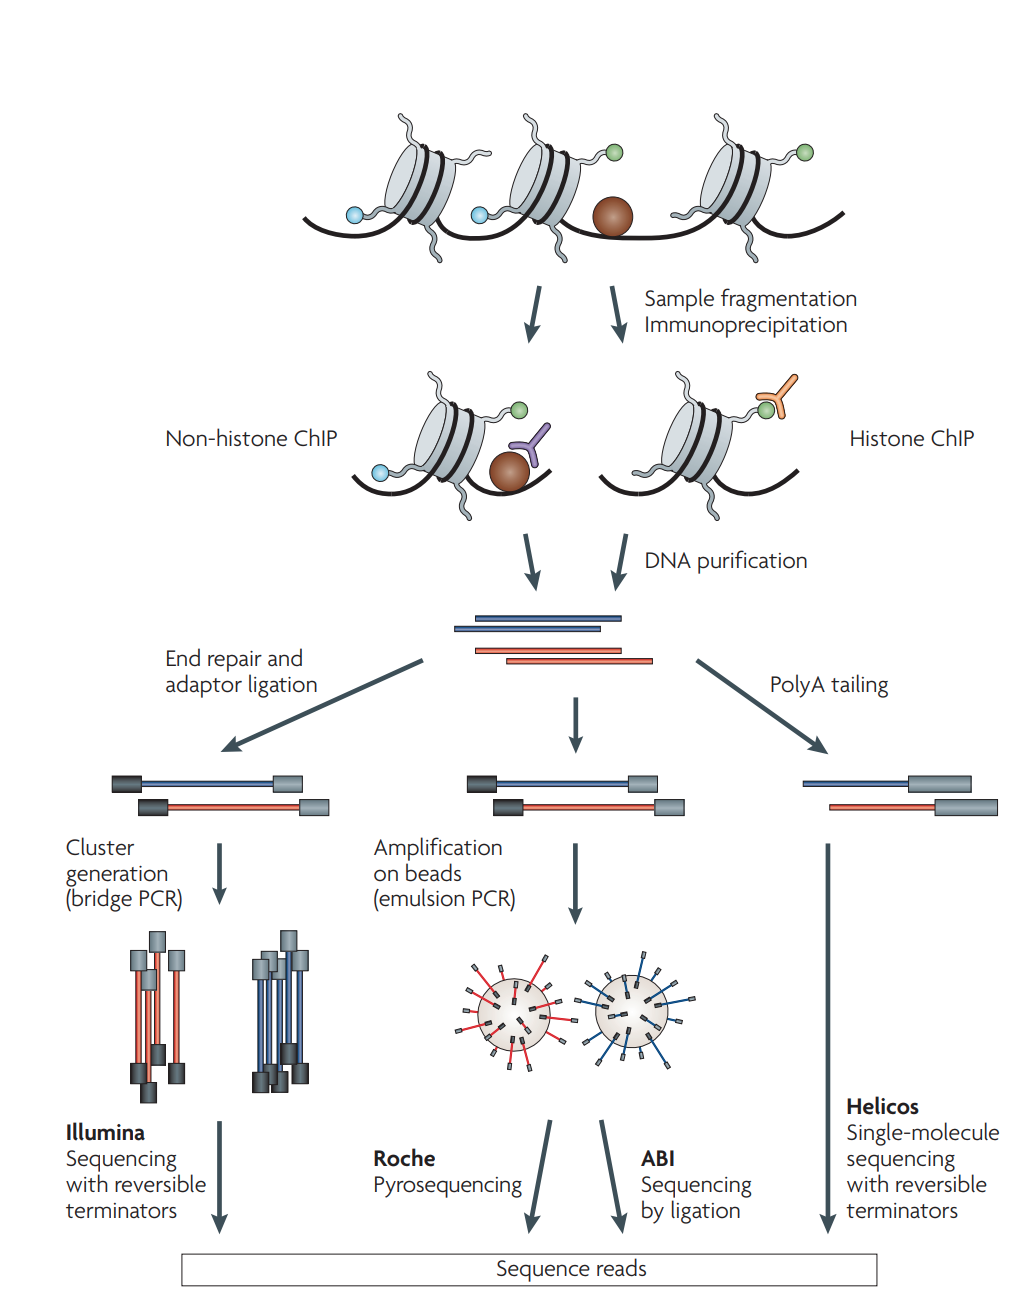
\includegraphics[width=0.4\linewidth]{figures/tf_measurement}
        \caption{How ChIP-seq (Chromatin Immunoprecipitation sequencing) works~\cite{Park2009-im}.}
        \label{fig:tf_explanation}
    \end{figure} 
\end{frame}

\begin{frame}[t]{Chromatin shape determines DNA transcription}
    \begin{figure}[htpb]
        \centering
        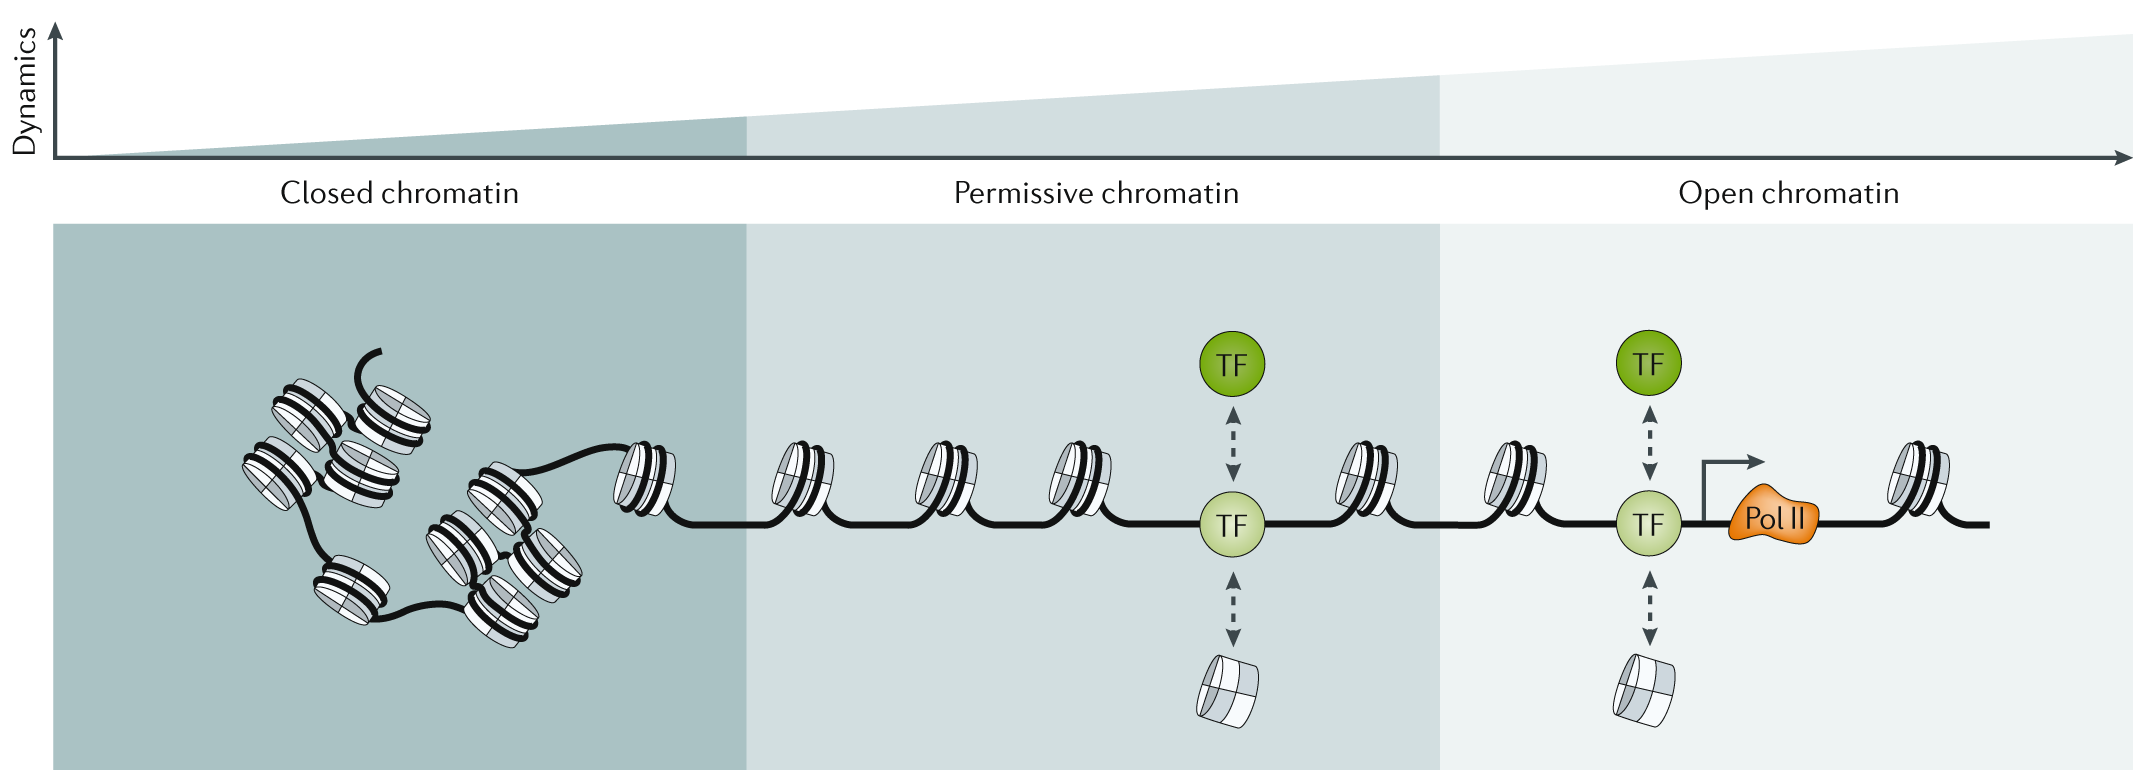
\includegraphics[width=0.8\linewidth]{figures/chrom_acc_explanation}
        \caption{Mechanism by which chromatin accessibility regulates transcription~\cite{Klemm2019-hk}.}
        \label{fig:figures/chrom_acc_explanation}
    \end{figure} 
\end{frame}

\begin{frame}[t]{Measuring chromatin accessibility}
    \begin{figure}[htpb]
        \centering
        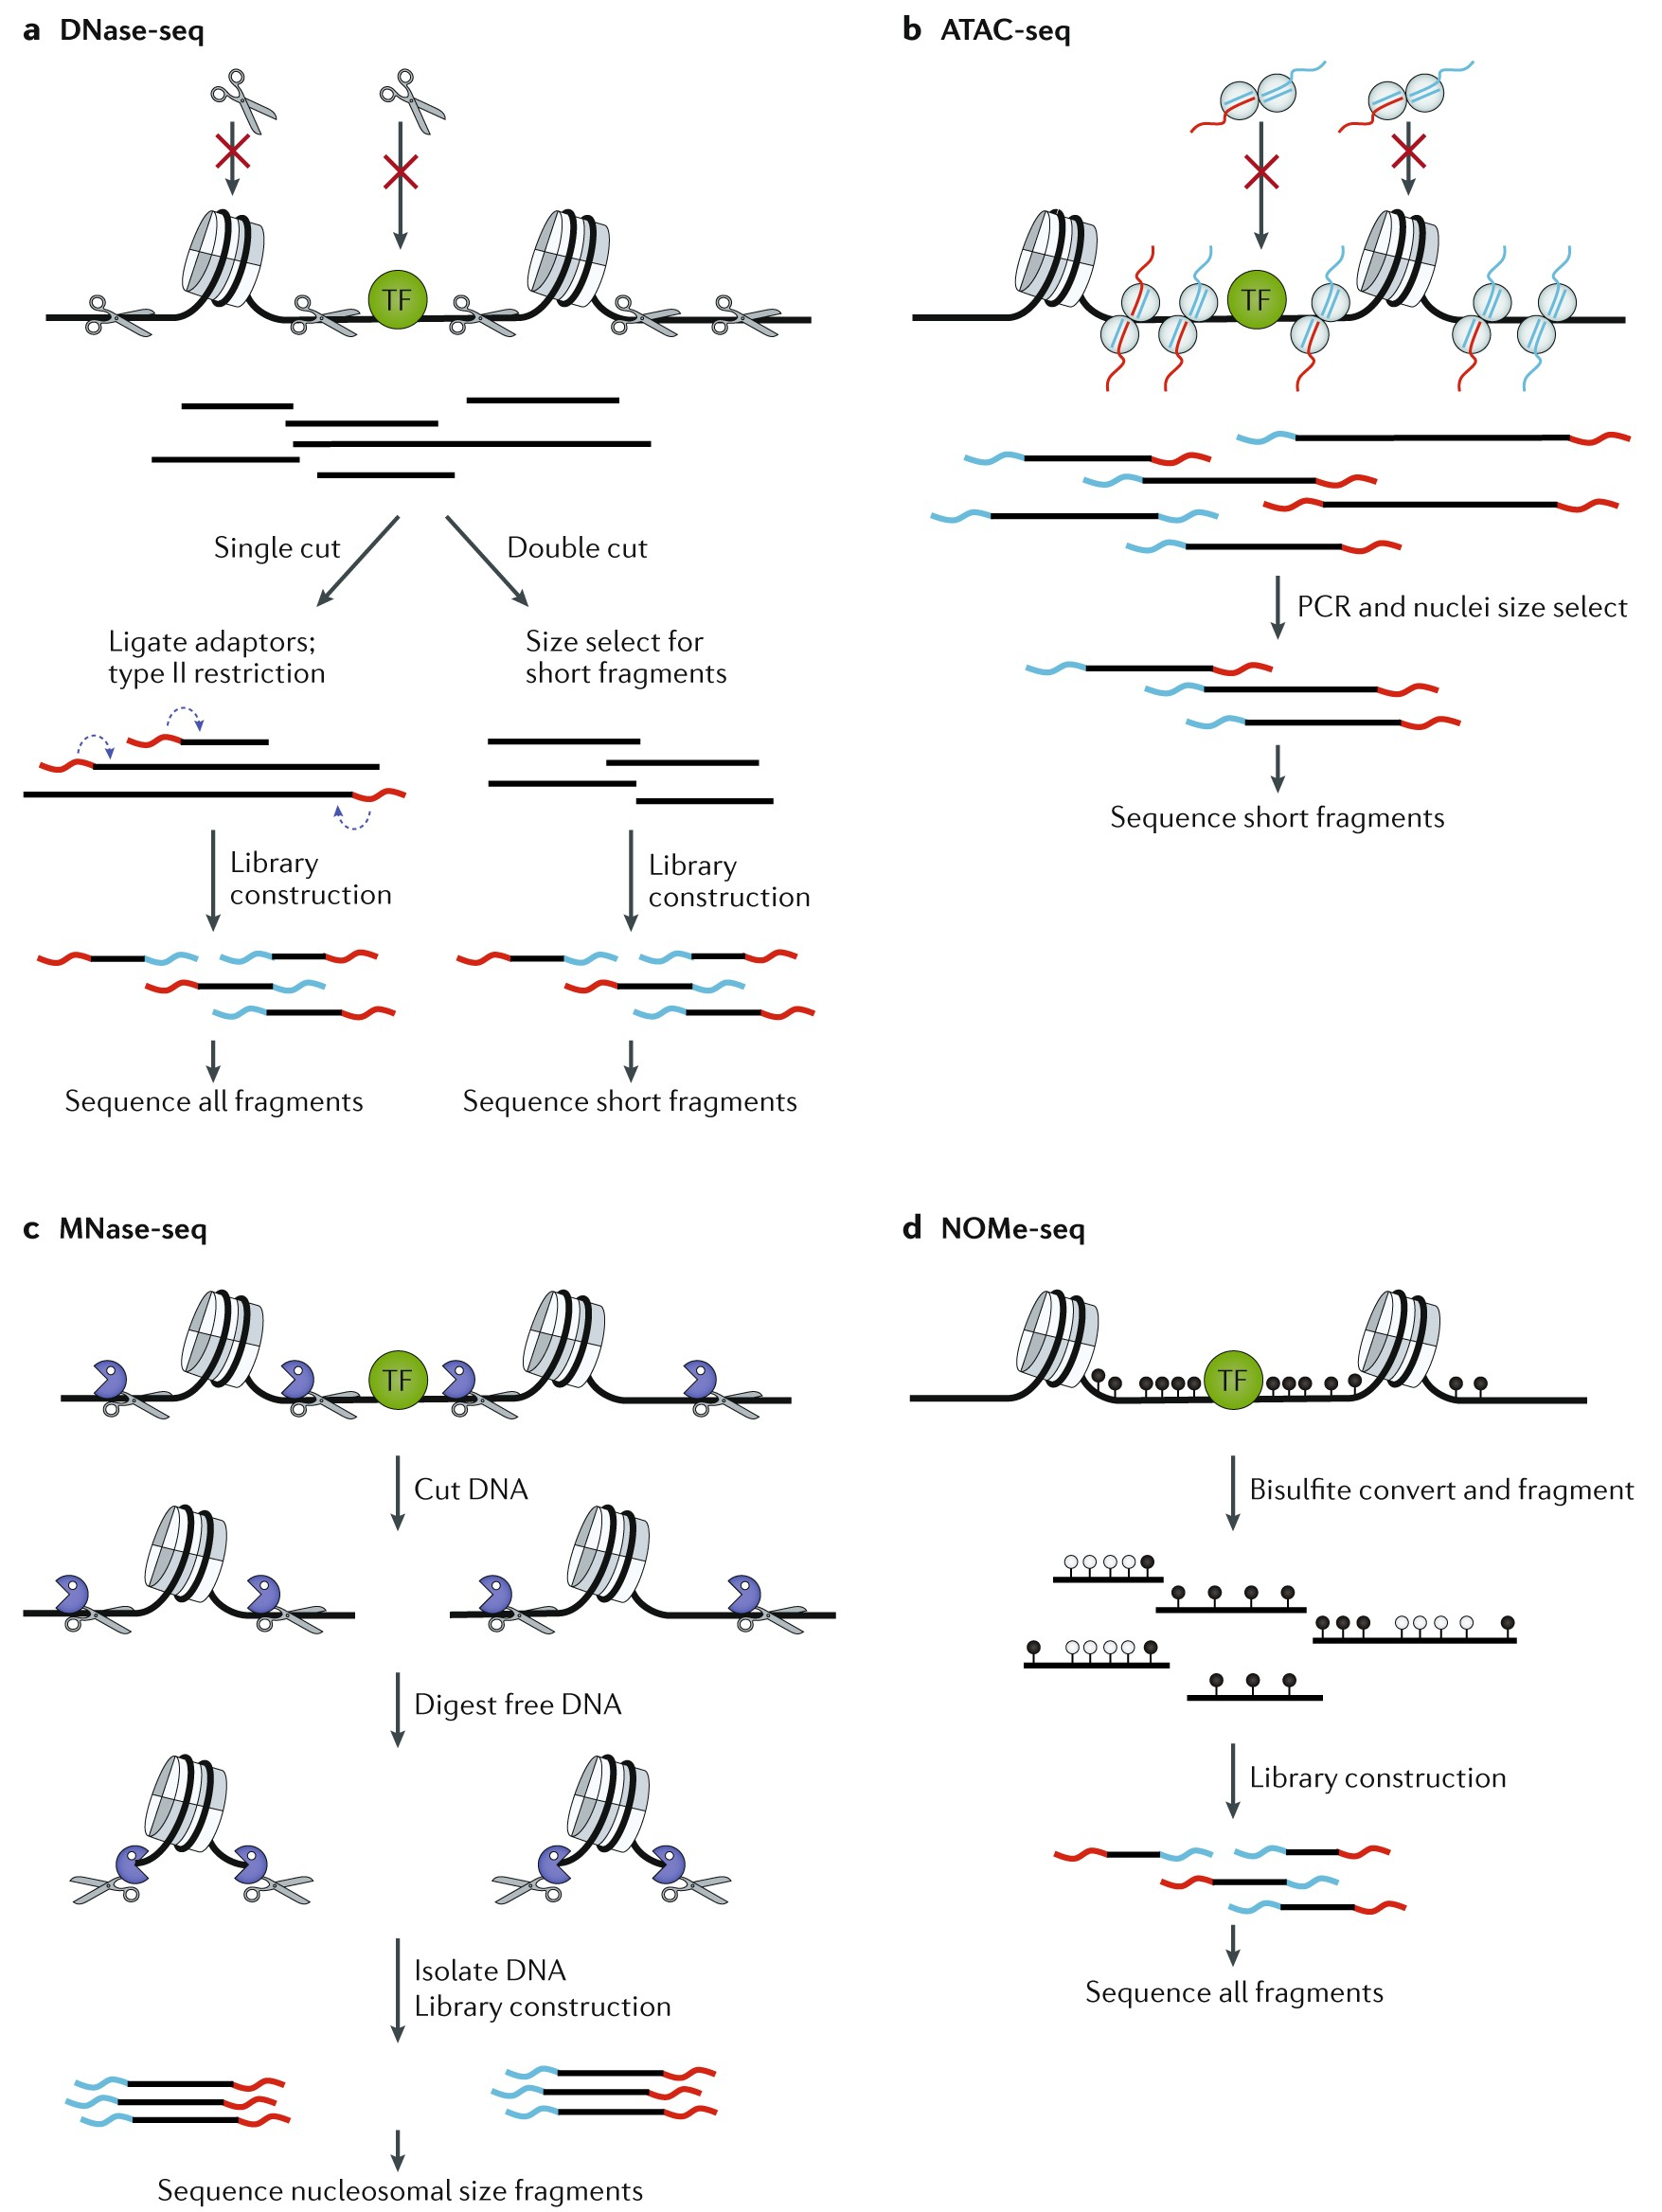
\includegraphics[width=0.4\linewidth]{figures/chrom_acc_measurement}
        \caption{Four methods for measuring chromatin accessibility~\cite{Klemm2019-hk}.}
        \label{fig:figures/chrom_acc_measurement}
    \end{figure} 
\end{frame}

\section{Methods}
\begin{frame}[t]{Questions we hope our method will answer}
    \begin{itemize}
        \item Do jointly trained models learn\footnote{Where `learn' is defined in terms of whether they can generate data that reflects them.} causal relationships?
        \item According to this model, does binding of a pioneer transcription factor causally influence chromatin accessibility (and vice versa)?
    \end{itemize}
\end{frame}

% \begin{frame}[t]{Terminology \& Notation}
% \begin{itemize}
%     \item \textit{Chromatin accessibility}: Chromatin is `accessible' if it's `open' as measured by the methods discussed above (in our case, DNase-seq).
%     \item \textit{Exposure}: The thing we believe is a `cause'. In all of what follows, this will be TF binding.
%     \item \textit{Outcome}: The thing we believe is an `effect'. In all of what follows, this will be chromatin accessibility (CA).
% \end{itemize}
% \end{frame}

\begin{frame}[t]{Intuition / Assumptions}
    \begin{itemize}
        \item Want to estimate whether one process (binding) causally influences another (accessibility) at the sequence region level and at the sequence population level
        \item If our model 'understands' causal relationships, we should be able to get it to generate data that reflects them
        \item ``Average causal effects'' is a meaningful concept at the sequence region and sequence population levels
    \end{itemize}
\end{frame}

\begin{frame}[t]{Step-by-step Overview}
    \begin{enumerate}
        \item Jointly train DL model to predict candidate cause(s) (`exposure') \& effect(s) (`outcome')
        \item Randomly sample sequences from held-out set and do in-silico saturation mutagenesis on each
            \begin{itemize}
                \item Generate exposure and outcome predictions using DL model
                \item Use MC dropout to generate standard errors for predictions
            \end{itemize}
        \item Treat difference between probabilities between each mutation and the reference sequence as effect size, analogous to a GWAS summary statistic
        \item Use MR to estimate average causal effects for each sequence
        \item Use meta-analysis method to aggregate causal effects across sequences
    \end{enumerate}
\end{frame}

\begin{frame}[t]{Details}
    To the whiteboard!
\end{frame}

\section{Preliminary Results}
\begin{frame}[t]{``Raw'' Data}
    \begin{figure}[htpb]
        \centering
        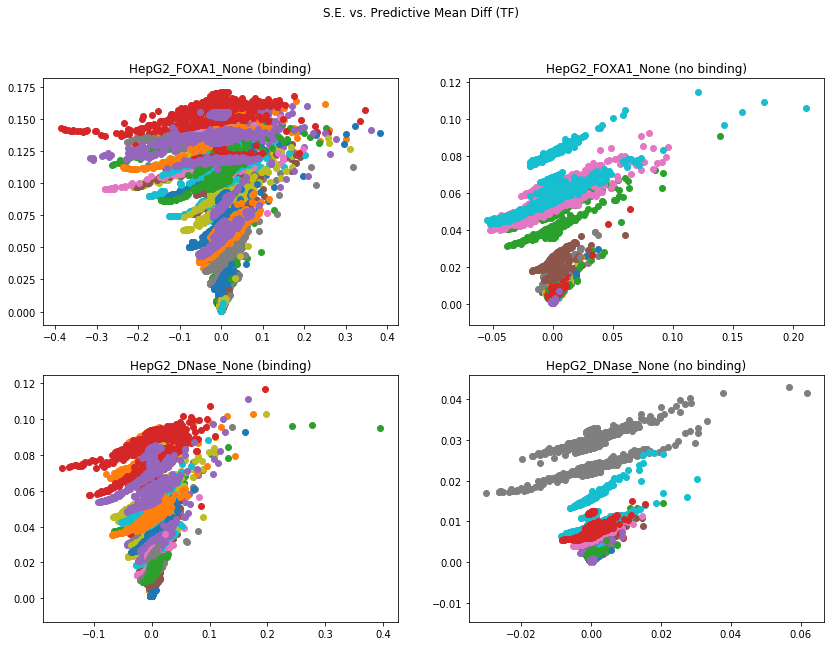
\includegraphics[scale=0.2]{figures/se_vs_predictive_mean_diff}
        \caption{Scatter plots of standard errors as a function of predictive mean for 50 randomly sampled sequences. Two top plots represent prediction for binding and non-binding sequences respectively. Two bottom plots are split same way for chromatin accessibility.}
        \label{fig:se_vs_predictive_mean_diff}
    \end{figure} 
\end{frame}

\begin{frame}[t]{Causal Effect Estimate Example}
    \begin{figure}[htpb]
        \centering
        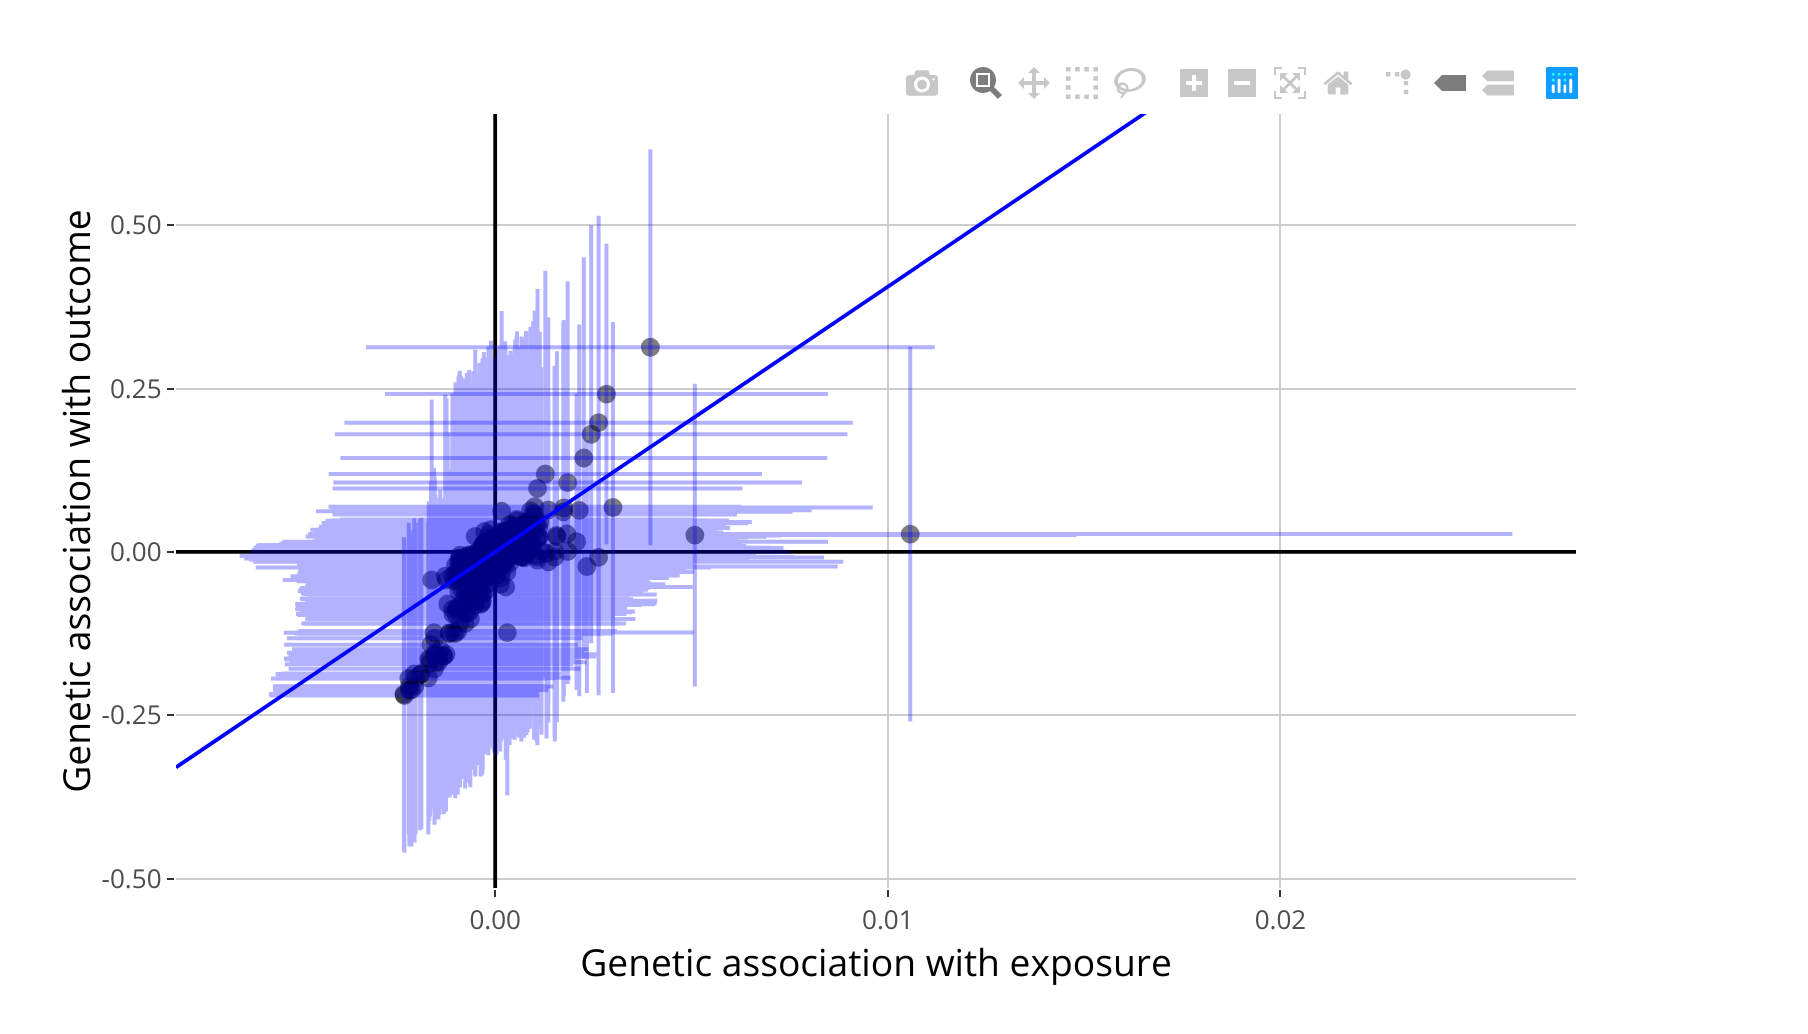
\includegraphics[scale=.15]{figures/egger_prelim_results}
        \caption{Preliminary results of running MR (Egger) for the predictions for a single sequence. The dots represent predictions for different mutation/reference pairs and the crosses standard errors.}
        \label{fig:egger_results_prelim}
    \end{figure} 
\end{frame}


\section{Limitations}

\begin{frame}[t]{Our deep net is deeply uncertain}
    \begin{block}{} Recall the preliminary results graphs. \end{block} 
    \begin{itemize}
        \item Our uncertainty (standard error) is too high, overwhelming any signal
        \item Seems like the network may be over-estimating its uncertainty
            \begin{itemize}
                \item \textbf{Intuition 1:} High accuracy should correlate with relatively low uncertainty
                \item \textbf{Intuition 2:} Similar to a probability distribution, uncertainty should have some normalizing factor
            \end{itemize}
        \item Can we test / fix the calibration of our uncertainty?
    \end{itemize}
\end{frame}

\begin{frame}[t]{Our deep net is deeply mis-calibrated}
    \begin{itemize}
        \item Calibration~\cite{Guo2017-qx}:
            \begin{itemize}
                \item Formally: \[ \Pr[\hat{y} = y \mid \hat{p} = p] =  p \]
                \item Semi-formally: our model assigns probability \( \hat{p} \) to \( (100 \times p) \)\% of samples with label 1
                \item Informally: if we look at all the sequences to which our model assigns high probability of label 1 (e.g. binding), most of them actually have label 1
            \end{itemize}
        \item Accuracy is not calibration (even with NLL loss)!
        \item DeepSEA is quite accurate but not very calibrated
    \end{itemize}
\end{frame}

\begin{frame}[t]{Our deep net is deeply mis-calibrated (cont.)}
    \begin{columns}
        \column{.5\textwidth}
        \begin{figure}
            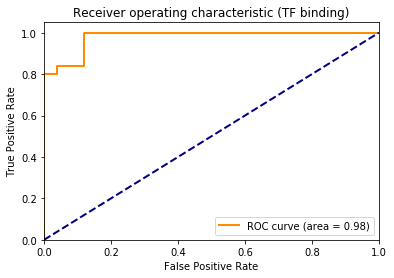
\includegraphics[scale=.4]{figures/deepsea_auc}
            \caption{DeepSEA AUC for randomly sampled sequences. Looking good!}
        \end{figure}
        \column{.5\textwidth}
        \begin{figure}
            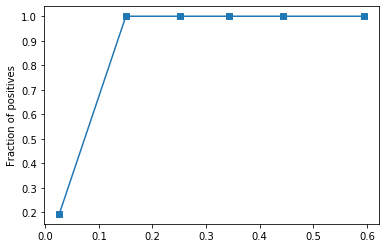
\includegraphics[scale=.4]{figures/deepsea_calibration}
            \caption{DeepSEA calibration for randomly sampled sequences. Not looking so good...}
        \end{figure}
    \end{columns}
\end{frame}

\begin{frame}[t]{Our deep net is deeply mis-calibrated (cont.)}
    \begin{block}{}
        What's really going on here?
    \end{block}
    \begin{columns}
        \column{.5\textwidth}
        \begin{figure}
            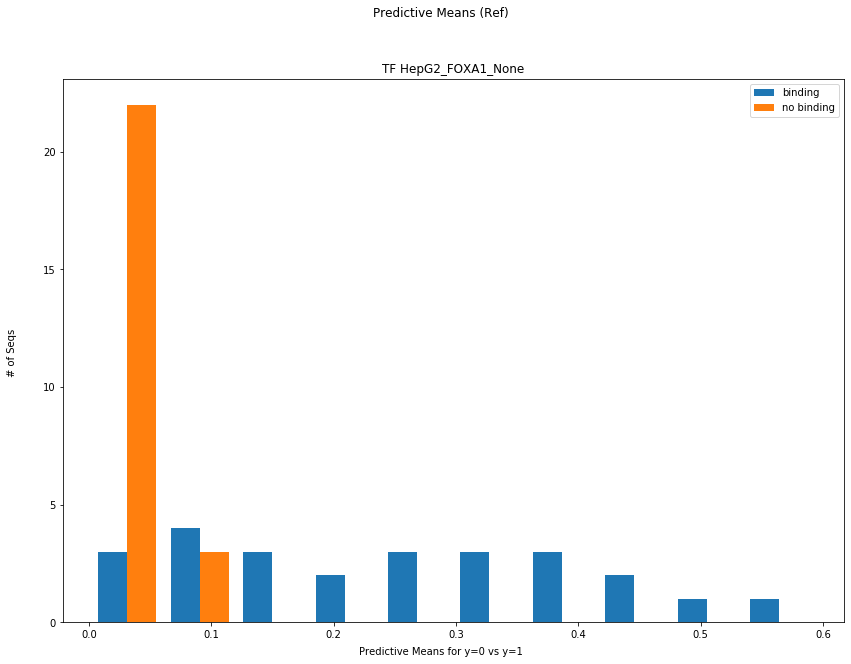
\includegraphics[scale=.2]{figures/predictive_mean_label_comparison}
            \caption{Histogram of binding probabilities. Note that overlap is low but really far to the left.}
        \end{figure}
        \column{.5\textwidth}
        \begin{figure}
            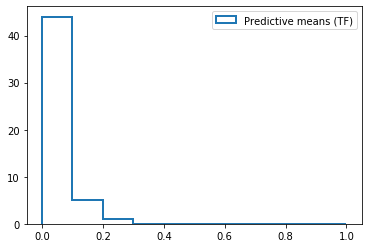
\includegraphics[scale=.4]{figures/deepsea_calibration_hist}
            \caption{DeepSEA calibration histogram for randomly sampled sequences. Not looking so good...}
        \end{figure}
    \end{columns}
\end{frame}

\section{Upcoming \& Future Work}
\begin{frame}[t]{Near Term Work}
    \begin{itemize}
        \item Measure calibration of uncertainty not just predictions
        \item Figure out whether we can calibrate DeepSEA without re-training it
            \begin{itemize}
                \item Isotonic regression
                \item Temperature scaling
            \end{itemize}
        \item Bayesian MR for mode-based estimator
    \end{itemize}
\end{frame}

\begin{frame}[t]{Long Term Work}
    \begin{itemize}
        \item Improve efficiency so can run for 1000s of sequences
        \item Learn a causal model directly (Deep IV~\cite{Hartford2017-cm})
    \end{itemize} 
\end{frame}

\section{Conclusion}
\begin{frame}[t]{If you only remember one slide...}
   \begin{block}{Goal}
        To go from models to mechanisms and hypotheses.
   \end{block} 
   \begin{block}{How to get there?}
       Methods for interrogating complex models and the \textbf{relationships} they learn at a higher level.
   \end{block}
   \begin{block}{Our contribution}
       Think of understanding what a network learns through the lens of causal inference. Focus on average effects rather than individual predictions.
   \end{block}

   Thank you!
\end{frame}

\begin{frame}[t]{Acknowledgements}
    Thank you to:
    \begin{itemize}
        \item David
        \item Brielin
        \item Udai
    \end{itemize}
    for all of your help!
\end{frame}

\begin{frame}[allowframebreaks]{Bibliography}
    \bibliography{bib}
\end{frame}


\end{document}
